\chapter{Beauchamp}

The daring attempt to rob the count was the topic of conversation
throughout Paris for the next fortnight. The dying man had signed a
deposition declaring Benedetto to be the assassin. The police had
orders to make the strictest search for the murderer. Caderousse’s
knife, dark lantern, bunch of keys, and clothing, excepting the
waistcoat, which could not be found, were deposited at the registry;
the corpse was conveyed to the morgue. The count told everyone that
this adventure had happened during his absence at Auteuil, and that he
only knew what was related by the Abbé Busoni, who that evening, by
mere chance, had requested to pass the night in his house, to examine
some valuable books in his library.

Bertuccio alone turned pale whenever Benedetto’s name was mentioned in
his presence, but there was no reason why anyone should notice his
doing so.

Villefort, being called on to prove the crime, was preparing his brief
with the same ardor that he was accustomed to exercise when required to
speak in criminal cases.

But three weeks had already passed, and the most diligent search had
been unsuccessful; the attempted robbery and the murder of the robber
by his comrade were almost forgotten in anticipation of the approaching
marriage of Mademoiselle Danglars to the Count Andrea Cavalcanti. It
was expected that this wedding would shortly take place, as the young
man was received at the banker’s as the betrothed.

Letters had been despatched to M. Cavalcanti, as the count’s father,
who highly approved of the union, regretted his inability to leave
Parma at that time, and promised a wedding gift of a hundred and fifty
thousand livres. It was agreed that the three millions should be
intrusted to Danglars to invest; some persons had warned the young man
of the circumstances of his future father-in-law, who had of late
sustained repeated losses; but with sublime disinterestedness and
confidence the young man refused to listen, or to express a single
doubt to the baron.

The baron adored Count Andrea Cavalcanti; not so Mademoiselle Eugénie
Danglars. With an instinctive hatred of matrimony, she suffered
Andrea’s attentions in order to get rid of Morcerf; but when Andrea
urged his suit, she betrayed an entire dislike to him. The baron might
possibly have perceived it, but, attributing it to a caprice, feigned
ignorance.

The delay demanded by Beauchamp had nearly expired. Morcerf appreciated
the advice of Monte Cristo to let things die away of their own accord.
No one had taken up the remark about the general, and no one had
recognized in the officer who betrayed the castle of Yanina the noble
count in the House of Peers.

Albert, however, felt no less insulted; the few lines which had
irritated him were certainly intended as an insult. Besides, the manner
in which Beauchamp had closed the conference left a bitter recollection
in his heart. He cherished the thought of the duel, hoping to conceal
its true cause even from his seconds. Beauchamp had not been seen since
the day he visited Albert, and those of whom the latter inquired always
told him he was out on a journey which would detain him some days.
Where he was no one knew.

One morning Albert was awakened by his valet de chambre, who announced
Beauchamp. Albert rubbed his eyes, ordered his servant to introduce him
into the small smoking-room on the ground floor, dressed himself
quickly, and went down.

He found Beauchamp pacing the room; on perceiving him Beauchamp
stopped.

“Your arrival here, without waiting my visit at your house today, looks
well, sir,” said Albert. “Tell me, may I shake hands with you, saying,
‘Beauchamp, acknowledge you have injured me, and retain my friendship,’
or must I simply propose to you a choice of arms?”

“Albert,” said Beauchamp, with a look of sorrow which stupefied the
young man, “let us first sit down and talk.”

“Rather, sir, before we sit down, I must demand your answer.”

“Albert,” said the journalist, “these are questions which it is
difficult to answer.”

“I will facilitate it by repeating the question, ‘Will you, or will you
not, retract?’”

“Morcerf, it is not enough to answer ‘yes’ or ‘no’ to questions which
concern the honor, the social interest, and the life of such a man as
Lieutenant-général the Count of Morcerf, peer of France.”

“What must then be done?”

\begin{figure}[ht]
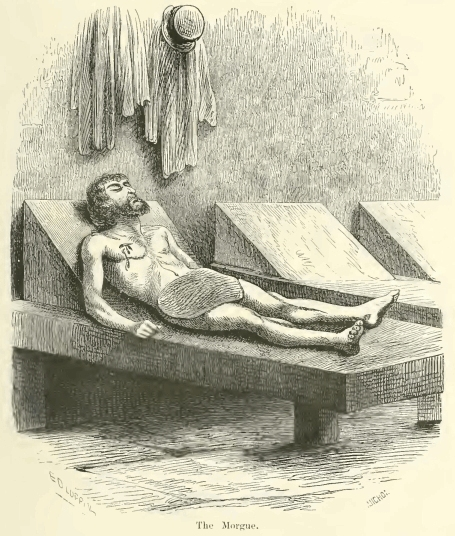
\includegraphics[width=\textwidth]{40174m.jpg}
\end{figure}

“What I have done, Albert. I reasoned thus—money, time, and fatigue are
nothing compared with the reputation and interests of a whole family;
probabilities will not suffice, only facts will justify a deadly combat
with a friend. If I strike with the sword, or discharge the contents of
a pistol at man with whom, for three years, I have been on terms of
intimacy, I must, at least, know why I do so; I must meet him with a
heart at ease, and that quiet conscience which a man needs when his own
arm must save his life.”

“Well,” said Morcerf, impatiently, “what does all this mean?”

“It means that I have just returned from Yanina.”

“From Yanina?”

“Yes.”

“Impossible!”

“Here is my passport; examine the visa—Geneva, Milan, Venice, Trieste,
Delvino, Yanina. Will you believe the government of a republic, a
kingdom, and an empire?” Albert cast his eyes on the passport, then
raised them in astonishment to Beauchamp.

“You have been to Yanina?” said he.

“Albert, had you been a stranger, a foreigner, a simple lord, like that
Englishman who came to demand satisfaction three or four months since,
and whom I killed to get rid of, I should not have taken this trouble;
but I thought this mark of consideration due to you. I took a week to
go, another to return, four days of quarantine, and forty-eight hours
to stay there; that makes three weeks. I returned last night, and here
I am.”

“What circumlocution! How long you are before you tell me what I most
wish to know?”

“Because, in truth, Albert——”

“You hesitate?”

“Yes,—I fear.”

“You fear to acknowledge that your correspondent has deceived you? Oh,
no self-love, Beauchamp. Acknowledge it, Beauchamp; your courage cannot
be doubted.”

“Not so,” murmured the journalist; “on the contrary——”

Albert turned frightfully pale; he endeavored to speak, but the words
died on his lips.

“My friend,” said Beauchamp, in the most affectionate tone, “I should
gladly make an apology; but, alas!——”

“But what?”

“The paragraph was correct, my friend.”

“What? That French officer——”

“Yes.”

“Fernand?”

“Yes.”

“The traitor who surrendered the castle of the man in whose service he
was——”

“Pardon me, my friend, that man was your father!”

Albert advanced furiously towards Beauchamp, but the latter restrained
him more by a mild look than by his extended hand.

“My friend,” said he, “here is a proof of it.”

\begin{figure}[ht]
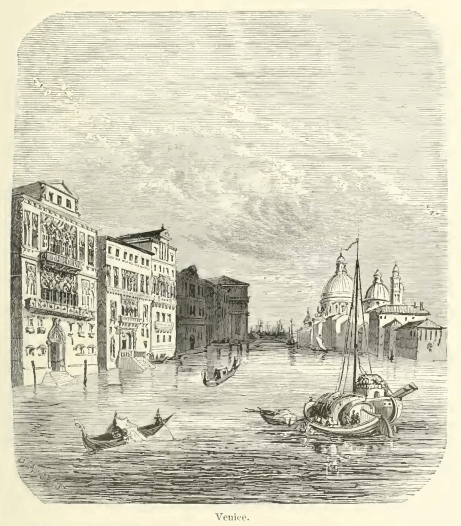
\includegraphics[width=\textwidth]{40176m.jpg}
\end{figure}

Albert opened the paper, it was an attestation of four notable
inhabitants of Yanina, proving that Colonel Fernand Mondego, in the
service of Ali Tepelini, had surrendered the castle for two million
crowns. The signatures were perfectly legal. Albert tottered and fell
overpowered in a chair. It could no longer be doubted; the family name
was fully given. After a moment’s mournful silence, his heart
overflowed, and he gave way to a flood of tears. Beauchamp, who had
watched with sincere pity the young man’s paroxysm of grief, approached
him.

“Now, Albert,” said he, “you understand me—do you not? I wished to see
all, and to judge of everything for myself, hoping the explanation
would be in your father’s favor, and that I might do him justice. But,
on the contrary, the particulars which are given prove that Fernand
Mondego, raised by Ali Pasha to the rank of governor-general, is no
other than Count Fernand of Morcerf; then, recollecting the honor you
had done me, in admitting me to your friendship, I hastened to you.”

Albert, still extended on the chair, covered his face with both hands,
as if to prevent the light from reaching him.

“I hastened to you,” continued Beauchamp, “to tell you, Albert, that in
this changing age, the faults of a father cannot revert upon his
children. Few have passed through this revolutionary period, in the
midst of which we were born, without some stain of infamy or blood to
soil the uniform of the soldier, or the gown of the magistrate. Now I
have these proofs, Albert, and I am in your confidence, no human power
can force me to a duel which your own conscience would reproach you
with as criminal, but I come to offer you what you can no longer demand
of me. Do you wish these proofs, these attestations, which I alone
possess, to be destroyed? Do you wish this frightful secret to remain
with us? Confided to me, it shall never escape my lips; say, Albert, my
friend, do you wish it?”

Albert threw himself on Beauchamp’s neck.

“Ah, noble fellow!” cried he.

“Take these,” said Beauchamp, presenting the papers to Albert.

Albert seized them with a convulsive hand, tore them in pieces, and
trembling lest the least vestige should escape and one day appear to
confront him, he approached the wax-light, always kept burning for
cigars, and burned every fragment.

“Dear, excellent friend,” murmured Albert, still burning the papers.

“Let all be forgotten as a sorrowful dream,” said Beauchamp; “let it
vanish as the last sparks from the blackened paper, and disappear as
the smoke from those silent ashes.”

“Yes, yes,” said Albert, “and may there remain only the eternal
friendship which I promised to my deliverer, which shall be transmitted
to our children’s children, and shall always remind me that I owe my
life and the honor of my name to you,—for had this been known, oh,
Beauchamp, I should have destroyed myself; or,—no, my poor mother! I
could not have killed her by the same blow,—I should have fled from my
country.”

“Dear Albert,” said Beauchamp. But this sudden and factitious joy soon
forsook the young man, and was succeeded by a still greater grief.

“Well,” said Beauchamp, “what still oppresses you, my friend?”

\begin{figure}[ht]
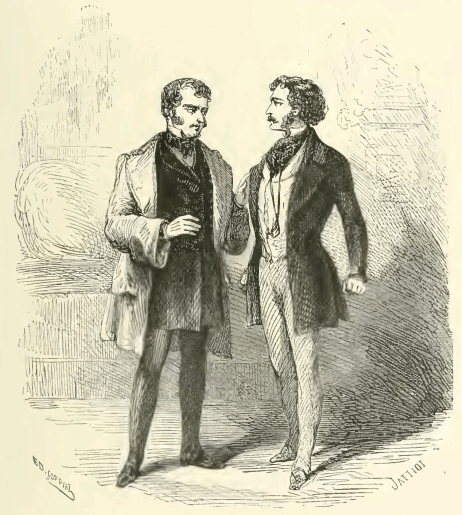
\includegraphics[width=\textwidth]{40178m.jpg}
\end{figure}

“I am broken-hearted,” said Albert. “Listen, Beauchamp! I cannot thus,
in a moment relinquish the respect, the confidence, and pride with
which a father’s untarnished name inspires a son. Oh, Beauchamp,
Beauchamp, how shall I now approach mine? Shall I draw back my forehead
from his embrace, or withhold my hand from his? I am the most wretched
of men. Ah, my mother, my poor mother!” said Albert, gazing through his
tears at his mother’s portrait; “if you know this, how much must you
suffer!”

“Come,” said Beauchamp, taking both his hands, “take courage, my
friend.”

“But how came that first note to be inserted in your journal? Some
unknown enemy—an invisible foe—has done this.”

“The more must you fortify yourself, Albert. Let no trace of emotion be
visible on your countenance, bear your grief as the cloud bears within
it ruin and death—a fatal secret, known only when the storm bursts. Go,
my friend, reserve your strength for the moment when the crash shall
come.”

\begin{figure}[ht]
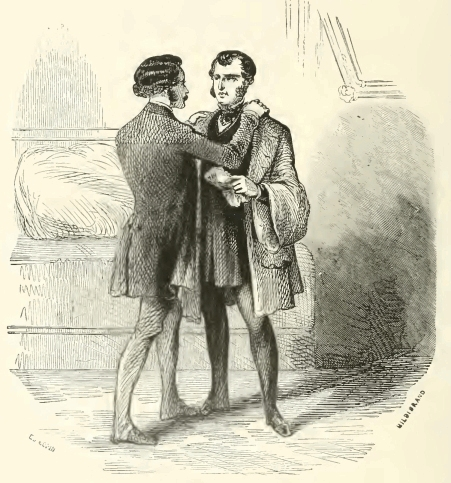
\includegraphics[width=\textwidth]{40179m.jpg}
\end{figure}

“You think, then, all is not over yet?” said Albert, horror-stricken.

“I think nothing, my friend; but all things are possible. By the way——”

“What?” said Albert, seeing that Beauchamp hesitated.

“Are you going to marry Mademoiselle Danglars?”

“Why do you ask me now?”

“Because the rupture or fulfilment of this engagement is connected with
the person of whom we were speaking.”

“How?” said Albert, whose brow reddened; “you think M. Danglars——”

“I ask you only how your engagement stands? Pray put no construction on
my words I do not mean they should convey, and give them no undue
weight.”

“No.” said Albert, “the engagement is broken off.”

“Well,” said Beauchamp. Then, seeing the young man was about to relapse
into melancholy, “Let us go out, Albert,” said he; “a ride in the wood
in the phaeton, or on horseback, will refresh you; we will then return
to breakfast, and you shall attend to your affairs, and I to mine.”

“Willingly,” said Albert; “but let us walk. I think a little exertion
would do me good.”

The two friends walked out on the fortress. When they arrived at the
Madeleine:

“Since we are out,” said Beauchamp, “let us call on M. de Monte Cristo;
he is admirably adapted to revive one’s spirits, because he never
interrogates, and in my opinion those who ask no questions are the best
comforters.”

“Gladly,” said Albert; “let us call—I love him.”
